\documentclass{standalone}
\usepackage[margin=1in]{geometry}
\usepackage[hang,small,bf]{caption}
\usepackage{tikz}
\usepackage{braket}
\usetikzlibrary{backgrounds,shadows.blur,fit,decorations.pathreplacing,shapes}

\begin{document}
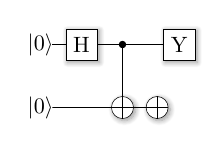
\begin{tikzpicture}[scale=0.8, transform shape]

\tikzstyle{basicshadow}=[blur shadow={shadow blur steps=8, shadow xshift=0.7pt, shadow yshift=-0.7pt, shadow scale=1.02}]\tikzstyle{basic}=[draw,fill=white,basicshadow]
\tikzstyle{operator}=[basic,minimum size=1.5em]
\tikzstyle{phase}=[fill=black,shape=circle,minimum size=0.1cm,inner sep=0pt,outer sep=0pt,draw=black]
\tikzstyle{none}=[inner sep=0pt,outer sep=-.5pt,minimum height=0.5cm+1pt]
\tikzstyle{measure}=[operator,inner sep=0pt,minimum height=0.5cm, minimum width=0.75cm]
\tikzstyle{xstyle}=[circle,basic,minimum height=0.35cm,minimum width=0.35cm,inner sep=-1pt,very thin]
\tikzset{
shadowed/.style={preaction={transform canvas={shift={(0.5pt,-0.5pt)}}, draw=gray, opacity=0.4}},
}
\tikzstyle{swapstyle}=[inner sep=-1pt, outer sep=-1pt, minimum width=0pt]
\tikzstyle{edgestyle}=[very thin]

\node[none] (line0_gate0) at (0.1,-0) {$\Ket{0}$};
\node[none] (line0_gate1) at (0.5,-0) {};
\node[none,minimum height=0.5cm,outer sep=0] (line0_gate2) at (0.75,-0) {};
\node[none] (line0_gate3) at (1.0,-0) {};
\draw[operator,edgestyle,outer sep=0.5cm] ([yshift=0.25cm]line0_gate1) rectangle ([yshift=-0.25cm]line0_gate3) node[pos=.5] {H};
\draw (line0_gate0) edge[edgestyle] (line0_gate1);
\node[none] (line1_gate0) at (0.1,-1) {$\Ket{0}$};
\node[xstyle] (line1_gate1) at (1.4000000000000001,-1) {};
\draw[edgestyle] (line1_gate1.north)--(line1_gate1.south);
\draw[edgestyle] (line1_gate1.west)--(line1_gate1.east);
\node[phase] (line0_gate4) at (1.4000000000000001,-0) {};
\draw (line0_gate4) edge[edgestyle] (line1_gate1);
\draw (line1_gate0) edge[edgestyle] (line1_gate1);
\draw (line0_gate3) edge[edgestyle] (line0_gate4);
\node[none] (line0_gate5) at (2.0500000000000003,-0) {};
\node[none,minimum height=0.5cm,outer sep=0] (line0_gate6) at (2.3000000000000003,-0) {};
\node[none] (line0_gate7) at (2.5500000000000003,-0) {};
\draw[operator,edgestyle,outer sep=0.5cm] ([yshift=0.25cm]line0_gate5) rectangle ([yshift=-0.25cm]line0_gate7) node[pos=.5] {Y};
\draw (line0_gate4) edge[edgestyle] (line0_gate5);
\node[xstyle] (line1_gate2) at (1.9500000000000002,-1) {};
\draw[edgestyle] (line1_gate2.north)--(line1_gate2.south);
\draw[edgestyle] (line1_gate2.west)--(line1_gate2.east);
\draw (line1_gate1) edge[edgestyle] (line1_gate2);

\end{tikzpicture}
\end{document}
